% vim: set spell spelllang=en tw=100 et sw=4 sts=4 :

\documentclass[a0paper]{tikzposter}

\usepackage{complexity}
\usepackage{wrapfig}
\usepackage{microtype}
\usepackage{gnuplot-lua-tikz}

\usepackage{lmodern}
\renewcommand*\familydefault{\sfdefault}
\usepackage[T1]{fontenc}

\title{Solving Hard Graph Problems in Parallel}
\author{Ciaran McCreesh and Patrick Prosser}
\institute{University of Glasgow, Glasgow, Scotland}
\titlegraphic{\includegraphics[keepaspectratio=true,scale=2.5]{UoG_keyline.pdf}}

\settitle{
    \begin{tikzpicture}
        \node (T) [inner sep=0pt] {\begin{minipage}{\linewidth}
                \color{titlefgcolor}
                {\bfseries \Huge \hspace{10mm}\@title \par}
                \vspace*{1em}
                {\Large {\bfseries \hspace{10mm}\@author}, \@institute}
        \end{minipage}};

        \node at (T.east) [anchor=center, inner sep=0pt, xshift=-8cm] {\@titlegraphic};
    \end{tikzpicture}
}

% University of Glasgow standard colours
\definecolor{uofguniversityblue}{rgb}{0, 0.219608, 0.396078}

\definecolor{uofgheather}{rgb}{0.356863, 0.32549, 0.490196}
\definecolor{uofgaquamarine}{rgb}{0.603922, 0.72549, 0.678431}
\definecolor{uofgslate}{rgb}{0.309804, 0.34902, 0.380392}
\definecolor{uofgrose}{rgb}{0.823529, 0.470588, 0.709804}
\definecolor{uofgmocha}{rgb}{0.709804, 0.564706, 0.47451}

\definecolor{uofglawn}{rgb}{0.517647, 0.741176, 0}
\definecolor{uofgcobalt}{rgb}{0, 0.615686, 0.92549}
\definecolor{uofgturquoise}{rgb}{0, 0.709804, 0.819608}
\definecolor{uofgsunshine}{rgb}{1.0, 0.862745, 0.211765}
\definecolor{uofgpumpkin}{rgb}{1.0, 0.72549, 0.282353}
\definecolor{uofgthistle}{rgb}{0.584314, 0.070588, 0.447059}
\definecolor{uofgpillarbox}{rgb}{0.701961, 0.047059, 0}
\definecolor{uofglavendar}{rgb}{0.356863, 0.301961, 0.580392}

\definecolor{uofgsandstone}{rgb}{0.321569, 0.278431, 0.231373}
\definecolor{uofgforest}{rgb}{0, 0.317647, 0.2}
\definecolor{uofgburgundy}{rgb}{0.490196, 0.133333, 0.223529}
\definecolor{uofgrust}{rgb}{0.603922, 0.227451, 0.023529}

\definecolorstyle{UofG}{
}{
    % Background Colors
    \colorlet{backgroundcolor}{uofgsandstone}
    \colorlet{framecolor}{black}
    % Title Colors
    \colorlet{titlefgcolor}{white}
    \colorlet{titlebgcolor}{uofguniversityblue}
    % Block Colors
    \colorlet{blocktitlebgcolor}{white}
    \colorlet{blocktitlefgcolor}{uofguniversityblue}
    \colorlet{blockbodybgcolor}{white}
    \colorlet{blockbodyfgcolor}{black}
    % Innerblock Colors
    \colorlet{innerblocktitlebgcolor}{uofguniversityblue}
    \colorlet{innerblocktitlefgcolor}{black}
    \colorlet{innerblockbodybgcolor}{uofgsandstone}
    \colorlet{innerblockbodyfgcolor}{black}
    % Note colors
    \colorlet{notefgcolor}{black}
    \colorlet{notebgcolor}{uofgrust}
    \colorlet{noteframecolor}{red}
}

\usetheme{Autumn}
\usecolorstyle{UofG}

\tikzposterlatexaffectionproofoff

\useblockstyle[bodyverticalshift=-1cm, roundedcorners=1]{Default}

\renewcommand{\Huge}{\fontsize{77.2}{96}\selectfont}

% Styles for drawings

\tikzset{edge/.style={line width=3pt, color=uofgsandstone}}
\tikzset{ledge/.style={line width=3pt, color=uofgsandstone!40!white}}

\begin{document}
\maketitle

{
    \colorlet{blockbodybgcolor}{uofgpumpkin}
    \colorlet{blocktitlebgcolor}{uofgpumpkin}
    \block[bodyverticalshift=0cm, bodyinnersep=3mm]{}{
        \centering\begin{minipage}{0.94\textwidth}
            \textbf{Graphs} allows us to model complex and dynamic relationships, and can be used to
            represent industrial \textbf{optimisation} and \textbf{scheduling} problems.  Our
            research investigates how we can \textbf{exploit parallelism} present in today's
            multi-core processors to speed up solving \NP-hard graph problems, or to allow us to
            tackle larger or more complicated problems in the time we have.
        \end{minipage}
    }
}

\begin{columns}
\column{0.5}

\block{Graph Colouring (Minimising Resource Usage)}{
\begin{wrapfigure}[8]{r}{0.38\linewidth}
    \begin{center}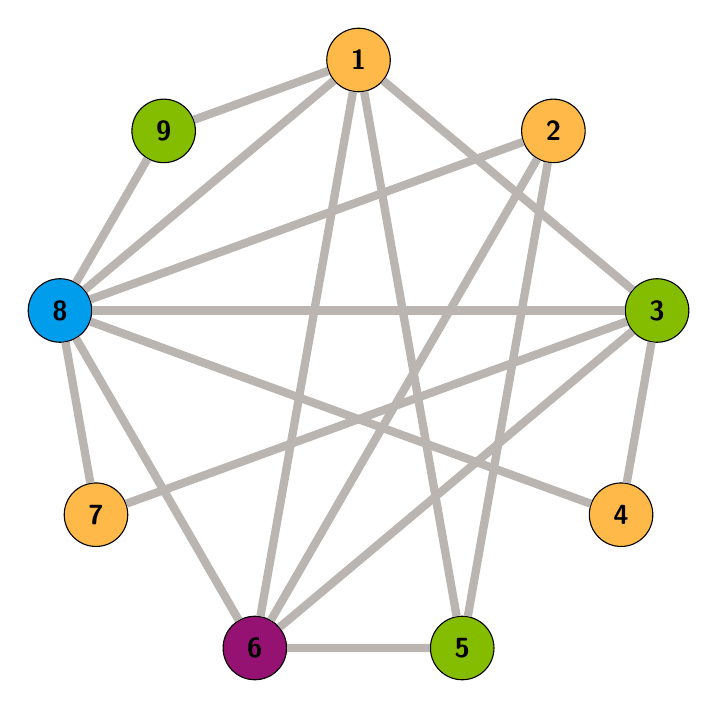
\begin{tikzpicture}[scale=1.75]%{{{
        \newcount \c
        \foreach \n in {1, ..., 9}{
            \c=\n
            \multiply\c by -40
            \advance\c by 130

            \ifthenelse{\n = 1 \OR \n = 2 \OR \n = 4 \OR \n = 7}{
                \node [draw, circle, fill=uofgpumpkin, inner sep=5pt, font=\bfseries] (N\n) at (\the\c:2.2) {\n};
            }{
                \ifthenelse{\n = 3 \OR \n = 5 \OR \n = 4 \OR \n = 7 \OR \n = 9}{
                    \node [draw, circle, fill=uofglawn, inner sep=5pt, font=\bfseries] (N\n) at (\the\c:2.2) {\n};
                }{
                    \ifthenelse{\n = 6}{
                        \node [draw, circle, fill=uofgthistle, inner sep=5pt, font=\bfseries] (N\n) at (\the\c:2.2) {\n};
                    }{
                        \node [draw, circle, fill=uofgcobalt, inner sep=5pt, font=\bfseries] (N\n) at (\the\c:2.2) {\n};
                    }
                }
            }
        }

        \draw [ledge] (N1) -- (N5); \draw [ledge] (N1) -- (N9);
        \draw [ledge] (N2) -- (N5); \draw [ledge] (N2) -- (N6); \draw [ledge] (N2) -- (N8);
        \draw [ledge] (N3) -- (N4); \draw [ledge] (N3) -- (N7);
        \draw [ledge] (N4) -- (N8);
        \draw [ledge] (N5) -- (N6);
        \draw [ledge] (N7) -- (N8);
        \draw [ledge] (N8) -- (N9);

        \draw [ledge] (N1) -- (N3);
        \draw [ledge] (N6) -- (N8);
        \draw [ledge] (N1) -- (N6);
        \draw [ledge] (N1) -- (N8);
        \draw [ledge] (N3) -- (N6);
        \draw [ledge] (N3) -- (N8);
    \end{tikzpicture}\end{center}
\end{wrapfigure}

Suppose we need to \textbf{schedule a day's meetings}. If a person needs to attend both meeting 3
and meeting 6, then these two meetings cannot be held at the same time. We can model this as a graph
problem: we draw a circle for each meeting, and put a line between two circles if these two meetings
must occur at different times. We then want to colour in these circles, giving adjacent circles
different colours, and using as few colours as possible. By treating different colours as different
time slots, colouring in the graph gives us an optimal meeting schedule.

\medskip

We can handle richer constraints: we might have a limit on how many circles any colour can be used
in (if we only have a \textbf{limited number of meeting rooms}), or we might want each colour to be
used on the same number of circles (for a \textbf{balanced workload}).

\medskip

More generally, graph colouring tells us how to use \textbf{as few resources as possible},
respecting conflicts. Industrial uses include call centre staff allocation, scheduling jobs on
machinery, radio bandwidth allocation, and reducing the impact of vehicle maintenance.
}

\block{Clique (Finding Groups of Mutual Friends)}{
\begin{wrapfigure}[8]{r}{0.38\linewidth}
    \begin{center}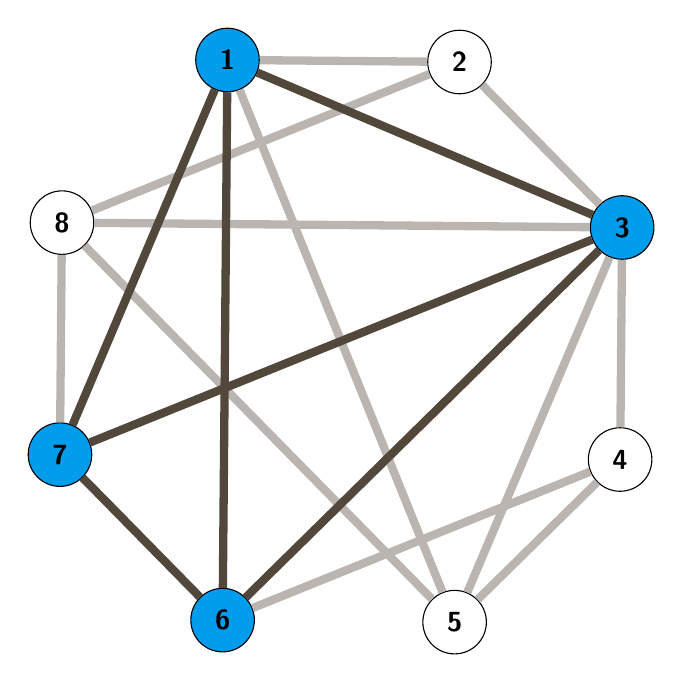
\begin{tikzpicture}[scale=1.75]%{{{
        \newcount \c
        \foreach \n in {1, ..., 8}{
            \c=\n \advance\c by -1 \multiply\c by -360 \divide\c by 8 \advance\c by 112.5
            \ifthenelse{\n = 1 \OR \n = 3 \OR \n = 6 \OR \n = 7}{
                \node[draw, circle, fill=uofgcobalt, inner sep=5pt, font=\bfseries] (N\n) at (\the\c:2.2) {\n};
            }{
                \node[draw, circle, fill=white, inner sep=5pt, font=\bfseries] (N\n) at (\the\c:2.2) {\n};
            }
        }

        \draw [ledge] (N1) -- (N2);
        \draw [ledge] (N1) -- (N5);
        \draw [ledge] (N2) -- (N3);
        \draw [ledge] (N2) -- (N8);
        \draw [ledge] (N3) -- (N4);
        \draw [ledge] (N3) -- (N5);
        \draw [ledge] (N3) -- (N8);
        \draw [ledge] (N4) -- (N5);
        \draw [ledge] (N4) -- (N6);
        \draw [ledge] (N5) -- (N8);
        \draw [ledge] (N7) -- (N8);

        \draw [edge] (N1) -- (N3);
        \draw [edge] (N1) -- (N6);
        \draw [edge] (N1) -- (N7);
        \draw [edge] (N3) -- (N6);
        \draw [edge] (N3) -- (N7);
        \draw [edge] (N6) -- (N7);
    \end{tikzpicture}\end{center}
\end{wrapfigure}

    A \textbf{clique} can be thought of as a group of people, where everyone in the group knows
    everyone else in the group.  Finding cliques lets us select \textbf{as much of a resource as
    possible}, respecting compatibility rules. Clique-finding algorithms have been used to improve
    the reliability of communications and networking protocols, for
    verifying electronic circuits, for social media analysis, for targeted advertising, and for controlling flying robots.
}

\block{Subgraph Isomorphism (Finding Patterns)}{
\begin{wrapfigure}[6]{r}{0.38\linewidth}
    \begin{center}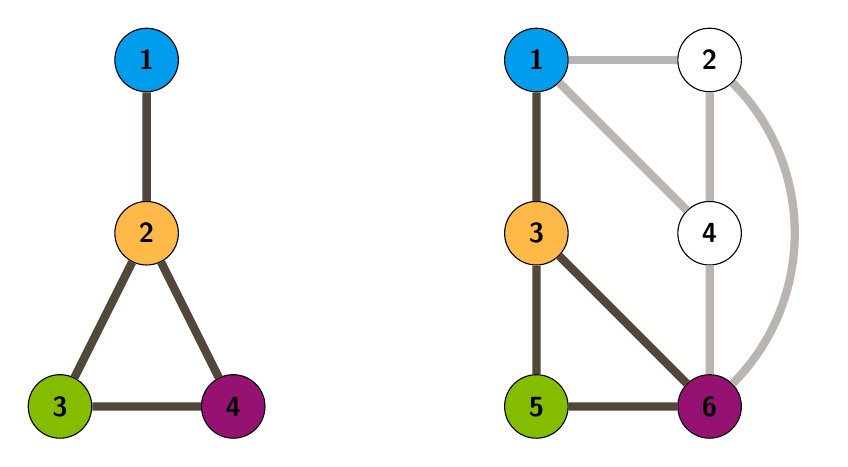
\begin{tikzpicture}[scale=1.1]%{{{
        \node[draw, circle, fill=uofgcobalt, inner sep=5pt, font=\bfseries] (Na) at (1,  0) {1};
        \node[draw, circle, fill=uofgpumpkin, inner sep=5pt, font=\bfseries] (Nb) at (1, -2) {2};
        \node[draw, circle, fill=uofglawn, inner sep=5pt, font=\bfseries] (Nc) at (0, -4) {3};
        \node[draw, circle, fill=uofgthistle, inner sep=5pt, font=\bfseries] (Nd) at (2, -4) {4};

        \draw [edge] (Na) -- (Nb);
        \draw [edge] (Nb) -- (Nc);
        \draw [edge] (Nc) -- (Nd);
        \draw [edge] (Nb) -- (Nd);

        \node[draw, circle, fill=uofgcobalt, inner sep=5pt, font=\bfseries] (N1) at (5.5,  0) {1};
        \node[draw, circle, fill=white, inner sep=5pt, font=\bfseries] (N2) at (7.5,  0) {2};
        \node[draw, circle, fill=uofgpumpkin, inner sep=5pt, font=\bfseries] (N3) at (5.5, -2) {3};
        \node[draw, circle, fill=white, inner sep=5pt, font=\bfseries] (N4) at (7.5, -2) {4};
        \node[draw, circle, fill=uofglawn, inner sep=5pt, font=\bfseries] (N5) at (5.5, -4) {5};
        \node[draw, circle, fill=uofgthistle, inner sep=5pt, font=\bfseries] (N6) at (7.5, -4) {6};

        \draw [ledge] (N1) -- (N2);
        \draw [edge] (N1) -- (N3);
        \draw [ledge] (N1) -- (N4);
        \draw [ledge] (N2) -- (N4);
        \draw [edge] (N3) -- (N5);
        \draw [edge] (N3) -- (N6);
        \draw [ledge] (N4) -- (N6);
        \draw [edge] (N5) -- (N6);
        \draw [ledge] (N2) to [in=45, out=315] (N6);

    \end{tikzpicture}\end{center}
\end{wrapfigure}

    Many real-world phenomena, such as social networks, transport routes, financial transactions,
    and chemical molecules, can be described using graphs. We may wish to \textbf{find interesting
    structures} inside these graphs. The subgraph isomorphism problem is to find a small ``pattern''
    graph in a big ``target'' graph. This is useful in drug design, in fraud detection, and in fault
    diagnosis.

    \medskip

    We can also \textbf{compare two graphs}. We do this via the maximum common subgraph problem,
    which is to find the largest subgraph common to two bigger graphs. This is useful in computer
    vision, database searches, and biochemistry.
}

\column{0.5}

\block{Backtracking and Backjumping Search as a Tree}{
    Practical algorithms for these problems combine inference (like you do when crossing out numbers
    when solving a Sudoku) and backtracking search (when we have to guess).  We may view the
    recursive calls made by a backtracking search algorithm as forming a tree:

    \vspace{0.5cm}
    \begin{center}
    \begin{tikzpicture}[scale=2.5]%{{{
        \coordinate (R);

        \coordinate (N) at (R);

        \coordinate (N1) at ($(N) + (-4, -0.75)$);
        \coordinate (N2) at ($(N) + ( 0, -0.75)$);
        \coordinate (N3) at ($(N) + ( 4, -0.75)$);

        \foreach \na in {1, ..., 3}{
            \coordinate (N\na 1) at ($(N\na) + (-1.25, -1)$);
            \coordinate (N\na 2) at ($(N\na) + ( 0,    -1)$);
            \coordinate (N\na 3) at ($(N\na) + ( 1.25, -1)$);

            \foreach \nb in {1, ..., 3}{
                \coordinate (N\na\nb t1) at ($(N\na\nb) + (-0.5, -1)$);
                \coordinate (N\na\nb t2) at ($(N\na\nb) + ( 0.5, -1)$);

                \coordinate (N\na\nb s1) at ($(N\na\nb) + (-0.3, -0.6)$);
                \coordinate (N\na\nb s2) at ($(N\na\nb) + ( 0.3, -0.6)$);

                \coordinate (N\na\nb h1) at ($(N\na\nb) + (-1.5, -3)$);
                \coordinate (N\na\nb h2) at ($(N\na\nb) + ( 1.5, -3)$);
            }
        }

        \foreach \na in {1, ..., 3}{
            \draw (N) -- (N\na);
            \foreach \nb in {1, ..., 3}{
                \draw (N\na) -- (N\na\nb);
            }
        }

        \tikzstyle{tf} = [draw, fill, fill=uofgcobalt, rounded corners];
        \tikzstyle{ts} = [draw, fill, fill=white, rounded corners];
        \foreach \na in {1, ..., 3}{
            \foreach \nb in {1, ..., 3}{
                \ifthenelse{\na = 1}{
                    \draw [tf] (N\na\nb) -- (N\na\nb t1) -- (N\na\nb t2) -- cycle;
                }{}

                \ifthenelse{\na = 2}{
                    \ifthenelse{\na\nb = 21}{
                        \draw [tf] (N\na\nb) -- (N\na\nb t1) -- (N\na\nb t2) -- cycle;
                    }{}
                    \ifthenelse{\na\nb = 22}{
                        \draw [tf] (N\na\nb) -- (N\na\nb t1) -- (N\na\nb t2) -- cycle;
                    }{}
                    \ifthenelse{\na\nb = 23}{
                        \draw [ts] (N\na\nb) -- (N\na\nb t1) -- (N\na\nb t2) -- cycle;
                    }{}
                }{}

                \ifthenelse{\na = 3}{
                    \draw [ts] (N\na\nb) -- (N\na\nb t1) -- (N\na\nb t2) -- cycle;
                }{}
            }
        }

        \tikzstyle{c} = [draw, circle, fill, fill=uofgcobalt];
        \tikzstyle{cf} = [draw, circle, fill, fill=uofgcobalt];
        \tikzstyle{cx} = [draw, forbidden sign, fill, fill=uofgcobalt];
        \tikzstyle{cs} = [draw, forbidden sign, fill, fill=white];
        \tikzstyle{cfs} = [draw, circle, fill, fill=white];
        \node [cx] at (N) { };

        \foreach \na in {1, ..., 3}{
            \ifthenelse{\na = 1}{
                \node [cx] at (N\na) { };
            }{}
            \ifthenelse{\na = 2}{
                \node [cf] at (N\na) { };
                \node [font=\scriptsize] at (N2) { $\uparrow$ };
            }{}
            \ifthenelse{\na = 3}{
                \node [cs] at (N\na) { };
            }{}

            \foreach \nb in {1, ..., 3}{
                \ifthenelse{\na = 1}{
                    \node [cx] at (N\na\nb) { };
                }{}

                \ifthenelse{\na = 2}{
                    \ifthenelse{\na\nb = 21}{
                        \node [cx] at (N\na\nb) { };
                    }{}
                    \ifthenelse{\na\nb = 22}{
                        \node [cf] at (N\na\nb) { };
                        \node [font=\scriptsize] at (N22) { $\uparrow$ };
                    }{}
                    \ifthenelse{\na\nb = 23}{
                        \node [cs] at (N\na\nb) { };
                    }{}
                }{}

                \ifthenelse{\na = 3}{
                    \ifthenelse{\na\nb = 31}{
                        \node [cfs] at (N\na\nb) { };
                        \node [font=\scriptsize] at (N31) { $\uparrow$ };
                    }{
                        \node [cs] at (N\na\nb) { };
                    }
                }{}
            }
        }
    \end{tikzpicture}%}}}
    \end{center}

    \vspace{0.5cm}

    A backtracking search algorithm is like a depth-first search over such a tree.  When a failure
    is encountered, we could just backtrack. \textbf{Backjumping} is a technique which sometimes
    allows us to backtrack several steps immediately. We show this as a $\uparrow$ symbol. This
    allows us to eliminate some subproblems based upon information discovered during search. This
    also happens in branch-and-bound algorithms for optimisation problems, where we dynamically
    eliminate subtrees which cannot beat the best solution found so far.
}

\block{Parallel Search: Work-Splitting Matters}{
    Viewing recursive calls as a tree, we can \textbf{evaluate sub-trees in parallel}. However,
    static decomposition leads to \textbf{poor work balance}, because we do not know up-front how
    large each subtree is.

    \vspace{1cm}

    \begin{center}
    \begin{tikzpicture}[scale=2.5]%{{{
        \coordinate (R);

        \coordinate (N) at (R);

        \coordinate (N1) at ($(N) + (-4, -0.75)$);
        \coordinate (N2) at ($(N) + ( 0, -0.75)$);
        \coordinate (N3) at ($(N) + ( 4, -0.75)$);

        \foreach \na in {1, ..., 3}{
            \coordinate (N\na 1) at ($(N\na) + (-1.25, -1)$);
            \coordinate (N\na 2) at ($(N\na) + ( 0,    -1)$);
            \coordinate (N\na 3) at ($(N\na) + ( 1.25, -1)$);

            \foreach \nb in {1, ..., 3}{
                \coordinate (N\na\nb t1) at ($(N\na\nb) + (-0.45, -1)$);
                \coordinate (N\na\nb t2) at ($(N\na\nb) + ( 0.45, -1)$);

                \coordinate (N\na\nb s1) at ($(N\na\nb) + (-0.25, -0.5)$);
                \coordinate (N\na\nb s2) at ($(N\na\nb) + ( 0.25, -0.5)$);

                \coordinate (N\na\nb h1) at ($(N\na\nb) + (-0.5, -1.4)$);
                \coordinate (N\na\nb h2) at ($(N\na\nb) + ( 0.5, -1.4)$);
            }
        }

        \tikzstyle{p} = [draw, rounded corners, dashed, color=uofgpumpkin, line width=3pt];
        \draw [p] ($(N11) + (-0.55, 0.51)$) -- ($(N12) + (0.55, 0.51)$) -- ($(N12) + (0.55, -1.5)$) -- ($(N11) + (-0.55, -1.5)$) -- cycle;
        \draw [p] ($(N13) + (-0.55, 0.51)$) -- ($(N21) + (0.55, 0.51)$) -- ($(N21) + (0.55, -1.5)$) -- ($(N13) + (-0.55, -1.5)$) -- cycle;
        \draw [p] ($(N22) + (-0.55, 0.51)$) -- ($(N23) + (0.55, 0.51)$) -- ($(N23) + (0.55, -1.5)$) -- ($(N22) + (-0.55, -1.5)$) -- cycle;
        \draw [p] ($(N31) + (-0.55, 0.51)$) -- ($(N33) + (0.55, 0.51)$) -- ($(N33) + (0.55, -1.5)$) -- ($(N31) + (-0.55, -1.5)$) -- cycle;

        \foreach \na in {1, ..., 3}{
            \draw (N) -- (N\na);
            \foreach \nb in {1, ..., 3}{
                \draw (N\na) -- (N\na\nb);
            }
        }

        \tikzstyle{t} = [draw, fill, fill=uofgcobalt, rounded corners];

        \draw [t] (N11) -- (N11s1) -- (N11s2) -- cycle;
        \draw [t] (N12) -- (N12s1) -- (N12s2) -- cycle;
        \draw [t] (N13) -- (N13s1) -- (N13s2) -- cycle;

        \draw [t] (N21) -- (N21t1) -- (N21t2) -- cycle;
        \draw [t] (N22) -- (N22h1) -- (N22h2) -- cycle;
        \draw [t] (N23) -- (N23s1) -- (N23s2) -- cycle;

        \draw [t] (N31) -- (N31s1) -- (N31s2) -- cycle;
        \draw [t] (N32) -- (N32t1) -- (N32t2) -- cycle;
        \draw [t] (N33) -- (N33s1) -- (N33s2) -- cycle;

        \tikzstyle{c} = [draw, circle, fill, fill=uofgcobalt];
        \node [c] at (N) { };

        \foreach \na in {1, ..., 3}{
            \node [c] at (N\na) { };

            \foreach \nb in {1, ..., 3}{
                \node [c] at (N\na\nb) { };
            }
        }
    \end{tikzpicture}%}}}
    \end{center}

    \vspace{0.5cm}

    We get around this by creating many \textbf{more subproblems than processors}, and distributing
    work dynamically using a queue. The coloured boxes show two ways we might do this.

    \vspace{0.5cm}

    \begin{center}
    \begin{tikzpicture}[scale=2.5]%{{{
        \coordinate (R);

        \coordinate (N) at (R);

        \coordinate (N1) at ($(N) + (-4, -0.75)$);
        \coordinate (N2) at ($(N) + ( 0, -0.75)$);
        \coordinate (N3) at ($(N) + ( 4, -0.75)$);


        \foreach \na in {1, ..., 3}{
            \coordinate (N\na 1) at ($(N\na) + (-1.25, -1)$);
            \coordinate (N\na 2) at ($(N\na) + ( 0,    -1)$);
            \coordinate (N\na 3) at ($(N\na) + ( 1.25, -1)$);

            \foreach \nb in {1, ..., 3}{
                \coordinate (N\na\nb t1) at ($(N\na\nb) + (-0.5, -1)$);
                \coordinate (N\na\nb t2) at ($(N\na\nb) + ( 0.5, -1)$);

                \coordinate (N\na\nb s1) at ($(N\na\nb) + (-0.3, -0.6)$);
                \coordinate (N\na\nb s2) at ($(N\na\nb) + ( 0.3, -0.6)$);

                \coordinate (N\na\nb h1) at ($(N\na\nb) + (-1.5, -3)$);
                \coordinate (N\na\nb h2) at ($(N\na\nb) + ( 1.5, -3)$);
            }
        }

        \tikzstyle{p} = [draw, rounded corners, dashed, color=uofgpumpkin, line width=3pt];
        \tikzstyle{q} = [draw, rounded corners, dashed, color=uofglawn, line width=3pt];

        \foreach \na in {1, ..., 3}{
            \foreach \nb in {1, ..., 3}{
                \draw [p] ($(N\na\nb) + (-0.55, 0.51)$) -- ($(N\na\nb) + (0.55, 0.51)$) --
                ($(N\na\nb) + (0.55, -1.5)$) -- ($(N\na\nb) + (-0.55, -1.5)$) -- cycle;
            }

            \draw [q] ($(N\na 1) + (-0.65, 1.31)$) -- ($(N\na 3) + (0.65, 1.31)$) --
            ($(N\na 3) + (0.65, -1.6)$) -- ($(N\na 1) + (-0.65, -1.6)$) -- cycle;
        }

        \foreach \na in {1, ..., 3}{
            \draw (N) -- (N\na);
            \foreach \nb in {1, ..., 3}{
                \draw (N\na) -- (N\na\nb);
            }
        }

        \tikzstyle{t} = [draw, fill, fill=uofgcobalt, rounded corners];
        \foreach \na in {1, ..., 3}{
            \foreach \nb in {1, ..., 3}{
                \draw [t] (N\na\nb) -- (N\na\nb t1) -- (N\na\nb t2) -- cycle;
            }
        }

        \tikzstyle{c} = [draw, circle, fill, fill=uofgcobalt];
        \node [c] at (N) { };

        \foreach \na in {1, ..., 3}{
            \node [c] at (N\na) { };

            \foreach \nb in {1, ..., 3}{
                \node [c] at (N\na\nb) { };
            }
        }

        \node [c] at (N21t1) { };
        \node at (N21t1) { $\star$ };
    \end{tikzpicture}%}}}
    \end{center}

    \vspace{0.5cm}

    Work splitting strategies do not just affect balance: above, if work is split between two
    processors using the green splitting strategy, the solution (marked $\star$) is found more
    quickly than if the work is split by the yellow strategy, even though yellow gives
    better balance.
}

\end{columns}

\block{Research Area: Practical Techniques for Solving Hard Problems in Parallel}{
\begin{wrapfigure}[15]{r}{0.38\linewidth}
    \begin{center}\begin{tikzpicture}
        \input{gen-graph-speedup}
    \end{tikzpicture}\end{center}
\end{wrapfigure}

    These graph problems are \textbf{hard} (like the famous \textbf{travelling salesman problem}):
    every additional item we add in can double the difficulty of finding a solution, so the time
    taken to solve a problem grows exponentially. In practice we can usually avoid this worst case
    by combining strong inference, symmetry breaking, carefully selected heuristics, and intelligent
    search, while learning from failure.  However, solving these problems can still take longer than
    we would like.

    \medskip

    Modern processors have at least two, and sometimes as many as fifteen, processing cores. We
    might hope that we could use these cores to make our programs \textbf{run faster}, or at least
    to \textbf{solve larger or harder problems} in the time we have.

    \medskip

    In general, we may do this by splitting problems up into evenly sized, independent pieces of
    work, which may be evaluated in parallel. However, combinatorial optimisation problems tend to
    be \textbf{highly irregular} (cannot be split into evenly sized pieces) and require
    \textbf{speculative parallelism} (the pieces have dependencies upon each other, and we must
    guess what the answer might be allow parallel evaluation).

    \medskip

    Despite this, our results are favourable: we can give substantial speedups to state-of-the-art
    algorithms. Our approach uses parallelism to explicitly \textbf{introduce diversity} into a
    search process to offset the weakest choices made by heuristics, so our parallel workers are
    reducing our commitment to potentially costly early mistakes. This is combined with late
    rebalancing, to give good work balance with low overheads and good scalability. Finally, we
    have shown how to treat backjumping as a ``fold with left-zero elements'', to allow parallel
    search without risking an absolute slowdown.
}

\def\bysame{\leavevmode\hbox to3em{\hrulefill}\thinspace}

\block{References}{
    \small
    Ciaran McCreesh, Patrick Prosser: A Parallel, Backjumping Subgraph Isomorphism Algorithm using
    Supplemental Graphs. Submitted to CP 2015. \\
    \bysame: The Shape of the Search Tree for the Maximum Clique Problem,
    and the Implications for Parallel Branch and Bound. ACM Transactions on Parallel Computing
    Volume 2 Issue 1 (2015). \\
    \bysame: A Parallel Branch and Bound Algorithm for the Maximum Labelled
    Clique Problem. Optimization Letters (2014). \\
    \bysame: Multi-Threading a State-of-the-Art Maximum Clique Algorithm.
    Algorithms 6(4): 618-635 (2013).
}

{
    \colorlet{blockbodybgcolor}{uofgsandstone}
    \colorlet{blocktitlebgcolor}{uofgsandstone}
    \block[bodyverticalshift=-0.5cm]{}{
        Second year PhD student, supervised by Patrick
        Prosser and David Manlove. SICSA research theme: modelling and abstraction. This work was
        supported by the Engineering and Physical Sciences Research Council [grant number
        EP/K503058/1]. \hfill \texttt{c.mccreesh.1@research.gla.ac.uk}
    }
}

\end{document}

